\documentclass[a4paper,12pt]{book}
\usepackage[utf8]{inputenc}
\usepackage[T1]{polski}
\usepackage{polski}
\usepackage{color}
\usepackage{helvet}
\usepackage{graphicx}
\usepackage{geometry}
\usepackage{titlesec}
\usepackage{indentfirst}
\usepackage{verbatim}
\usepackage{moreverb}
\usepackage{nameref}
\usepackage[font=footnotesize,labelfont=bf]{caption}
\geometry{hmargin={2cm, 2cm}, height=10.0in}
\assignpagestyle{\chapter}{empty}
\newcommand{\param}[1]{\textit{\textless #1\textgreater}}
\title{System IPS opaty o iptables}
\author{Marcin TORGiren Fabrykowski}
\setcounter{secnumdepth}{4}
\setcounter{tocdepth}{4}
\begin{document}
\thispagestyle{empty}

\includegraphics[height=37.5mm]{agh_nzw_a_pl_1w_wbr_cmyk.eps}\\
\rule{30mm}{0pt}
{\large\textsf{Wydział Fizyki i Informatyki Stosowanej}}\\
\rule{\textwidth}{3pt}\\
\rule[2ex]
{\textwidth}{1pt}\\
\vspace{7ex}
\begin{center}
{\bf\LARGE\textsf{Praca inżynierska}}\\
\vspace{13ex}
% --------------------------- IMIE I NAZWISKO -------------------------------
{\bf\Large\textsf{Marcin Fabrykowski}}\\
\vspace{3ex}
{\sf \small kierunek studiów:} {\bf\small\textsf{informatyka stosowana}}\\
\vspace{15ex}
%% ------------------------ TYTUL PRACY --------------------------------------
{\bf\huge\textsf{System IPS oparty o iptables}}\\
\vspace{14ex}
%% ------------------------ OPIEKUN PRACY ------------------------------------
{\sf \Large Opiekun:} {\bf\Large\textsf{dr inż. Krzysztof Rzecki}}\\
\vspace{22ex}
\textsf{\bf\large\textsf{Kraków, styczeń 2013}}
\end{center}
%% =====  STRONA TYTUŁOWA PRACY INŻYNIERSKIEJ  ====

\newpage

%% =====  TYŁ STRONY TYTUŁOWEJ PRACY INŻYNIERSKIEJ  ====
{\sf Oświadczam, świadomy(-a) odpowiedzialności karnej za poświadczenie nieprawdy, że niniejszą pracę dyplomową wykonałem(-am) osobiście i samodzielnie i nie korzystałem(-am) ze źródeł innych niż wymienione w pracy.}

\vspace{14ex}

\begin{center}
\begin{tabular}{lr}
~~~~~~~~~~~~~~~~~~~~~~~~~~~~~~~~~~~~~~~~~~~~~~~~~~~~~~~~~~~~~~~~~ &
................................................................. \\
~ & {\sf (czytelny podpis)} \\
\end{tabular}
\end{center}

\newpage
\linespread{1.3}
\selectfont

\noindent
Na kolejnych dwóch stronach proszę dołączyć kolejno recenzje pracy popełnione przez Opiekuna oraz Recenzenta (wydrukowane z systemu MISIO i podpisane przez odpowiednio Opiekuna i Recenzenta pracy). Papierową wersję pracy (zawierającą podpisane recenzje) proszę złożyć w dziekanacie celem rejestracji.

\vspace{85mm}
\tableofcontents
\chapter*{Wstęp}
	\addcontentsline{toc}{chapter}{Wstęp}
\chapter{O IPS}
	\section{Co to jest IPS}
	System IPS (ang. Intrusion Prevention System) jest to system wykrywania i blokowania ataków sieciowych.
	Jego zadanie polega na analizie ruchu sieciowego wchodzącego do oraz przechodzącego przez niego oraz odpowiednie reagowanie w przypadku wykrycia nienormalnych zachowań sieci.
	\section{Schemat działania}
		\begin{enumerate}
			\item Analiza ruchu sieciowego
			\item Wykrycie zachowań pasujących do zdefiniowanych reguł bezpieczeństwa
			\item Reakcja na wykryte niebezpieczne zachowanie
			\item Poinformowanie administratora o próbie ataku oraz podjętych działaniach
			\item Zapisanie danych o ataku oraz podjętych działaniach do bazy danych
			\item Udostępnienie administratorowi wglądu w historię ataków
		\end{enumerate}
\chapter{Analiza ruchu sieciowego}
	\section{Używane narzędzie}
		Jako systemu analizującego ruch sieciowy wykorzystam pakiet Netfilter konfigurowany za pomocą iptables.
	\section{Netfilter}
		\subsection{Ogólny zarys}
			Netfilter jest oprogramowaniem pozwalającym na filtrowanie pakietów, ich translacje (NAT) oraz inne manipulację.
			Od wersji jądra 2.4.x, pakiet netfilter jest umieszczony wewnątrz niego.
			Potrafi on dopasowywać analizowane pakiety ze względu na szeroką gamę kryteriów, jak również przeprowadzić szereg operacji na danych pakietach.
		\subsection{Zasada działania}
			Netfilter posiada 4 zdefiniowane tablice: raw, mangle, nat, filter, oraz 5 łańcuchów: PREROUTING, INPUT, FORWARD, OUTPUT, POSTROUTING.
			Kolejność przechodzenia pakietu przez tabele i łańcuchy obrazuje rys. \ref{fig:flowchart}.\\
			\begin{figure}[h]
				\centering
					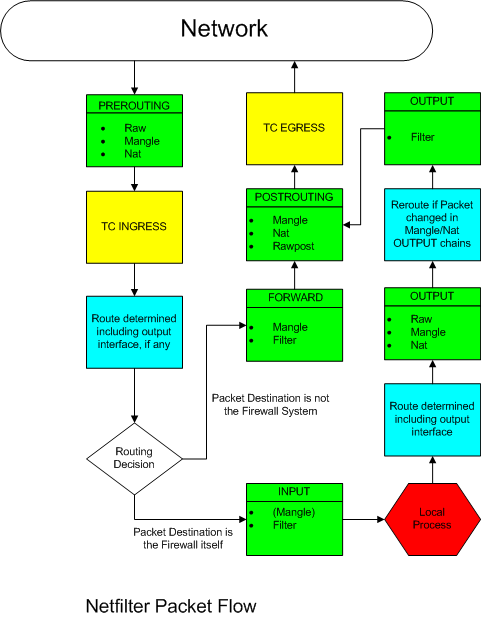
\includegraphics[width=280px]{Netfilter.png}
					\caption{Przepływ pakietów w netfilter}
					%http://www.shorewall.net/images/Netfilter.png
					\label{fig:flowchart}
			\end{figure}
			Gdy pakiet dochodzi do komputera na którym jest netfilter, zostaje on przekazany do łańcucha PREROUTING. Następnie, następuje decyzja o routowaniu pakietu, i w zależności czy pakiet jest kierowany do lokalnego komputera, jest kierowany do łańcucha INPUT, bądź w przypadku gdy ma zostać przekazany dalej, do łańcucha FORWARD oraz POSTROUTING.\\
			W przypadku, gdy pakiet jest generowany przez nasz komputer, zostaje on przejęty przez łańcuch OUTPUT, a następnie POSTROUTING.

			Pierwszą tablicą przez którą przechodzi pakiet, jest tablica \textit{raw}. W tym miejscu możemy oznaczyć pakiet targetem TRACE, który spowoduje logowanie każdej reguły do której pakiet będzie pasował. Wykorzystywane jest to przy debugowaniu sieci bądź firewalla.
			Inna opcją która może pojawić się jedynie w tablicy raw, jest target NOTRACK. Spowoduje on nieoznaczenie pakietu przez moduł \textit{conntrack}, który rejestruje pakiety i rozpoznaje je jako istniejące połączenia.

			Następna tablicą do której zostaje przekazany pakiet, jest tablica \textit{mangle}.
			W tablicy tej możemy manipulować wartościami TTL.

			Kolejną tablicą przetwarzającą pakiet, jest tablica \textit{nat}.
			W tablicy tej możemy manipulować adresami pakietowymi.
			W zależności, czy naszym celem jest SNAT cz DNAT, używamy do tego odpowiednich łańcuchów PREROUTING i POSTROUTING

			Ostatnią tablicą, która przetwarza pakiety, jest tablica \textit{filter}. Jest to tablica w której powinno się umieszczać wszystkie reguły dotyczące filtrowania pakietów. 
			Jeżeli nie zostanie jawnie podana tablica, domyślną tablicą jest tablica \textit{filter}.

			Jeżeli pakiet zostanie przetworzony przez całą ścieżkę w firewallu i nie zostanie podjęta decyzja o zaakceptowaniu bądź odrzuceniu pakietu, zostaje zastosowana polityka odpowiedniego dla tego pakietu łańcucha głównego, tj. INPUT, OUTPUT, FORWARD.
			Politykami mogą być TARGET-y terminujące, tj. ACCEPT, REJECT, DROP.
		\subsection{Najważniejsze kryteria dopasowania}
			Netfilter posiada bogaty wachlarz możliwości dopasowywania pakietów
			\begin{description}
				\item[-{}-source, -{}-src, -s \param{adres} ] \hfill \\
					dopasowuje adres źródłowy pakietu do podanego jako \textit{adres}
				\item[-{}-destination, -{}-dst, -d \param{adres}] \hfill\\
					dopasowuje adres docelowy pakietu do podanego jako \textit{adres}
				\item[-{}-protocol, -p \textit{\textless protocol \textgreater}] \hfill \\
					dopasowuje protokół używany przez pakiet.\\
					Najczęściej używane protokołu to: \textit{tcp},\textit{udp},\textit{icmp}
				\item[-{}-source-port, -{}-sport \textit{\textless port \textgreater} ]\hfill\\
					dopasowuje port źródłowy pakietu.\\
					Aby użyć tego dopasowania należy zdefiniować protokół.
				\item[-{}-destination-port, -{}-dport \textit{\textless port \textgreater}] \hfill \\
					dopasowuje port docelowy pakietu.\\
					Aby użyć tego dopasowania należy zdefiniować protokół.
				\item[-{}-tcp-flags \textit{\textless maska \textgreater \textless flagi \textgreater}] \hfill \\
					\textcolor{red}{\Large{DO POPRAWY STYLISTYCZNEJ}}\\
					dopasowuje pakiet, jeżeli wszystkie \textit{flagi} są ustawione, oraz wszystkie flagi wymienione w \textit{masce} oraz niewymienione w \textit{flags} są nieustawione
				\item[-{}-mac-source \textit{\textless mac-adres \textgreater}] \hfill \\
					dopasowuje pakiet na podstawie źródłowego adresu sieciowego. Adres podawany jest w formacie: AA:BB:CC:DD:EE:FF.
				\item[-{}-in-interface, -i \param{interface}] \hfill \\
					dopasowuje pakiet ze względu na interface sieciowy na którym dany pakiet się pojawił	
				\item[-{}-out-interface, -o \param{interface}] \hfill \\
					dopasowuje pakiet ze względu na interface sieciowy przez który pakiet będzie wysyłany
				\item[-{}-limit \param{ilość}/\param{czas}] \hfill \\
					dopasowuje pakiety, jeśli ich ilość nie przekracza \textit{ilość} w okresie \textit{czas}.\\
					\textit{Czas} może przyjmować wartości: second, minute, hour, day.
			\end{description}
		\subsection{Najważniejsze działania}
			Jeżeli pakiet zostanie dopasowany, netfilter może wykonać jedną ze zdefiniowanych akcji a pakiecie. W przypadku niezdefiniowania akcji, pakiet przechodzi do kolejnych reguł w firewallu a w firewallu zostaje zwiększony licznik dopasowanych pakietów dla danej reguły.\\
			Dopasowany pakiet zostaje wysłany do wybranego targetu poprzez opcję -j, np: -j~ACCEPT.
			\begin{description}
				\item[ACCEPT] \hfill \\
					dany pakiet zostaje zaakceptowany i nie przechodzi przez dalszą filtrację
				\item[REJECT] \hfill \\
					odrzucenie pakietu z wysłaniem informacji do adresata. Domyślna wartość odpowiedzi to icmp-port-unreachable.\\
					Istnieje możliwość ustawienia odpowiedzi wysyłanej do adresata poprzez atrybut -{}-reject-with \param{type},
					gdzie \textit{type} jest jednym z zdefiniowanych komunikatów:
					\begin{itemize}
						\item icmp-net-unreachable
						\item icmp-host-unreachable
						\item icmp-port-unreachable
						\item icmp-prot-unreachable
						\item icmp-net-prohibited
						\item icmp-host-prohibited
						\item icmp-admin-prohibited.
					\end{itemize}
				\item[DROP] \hfill \\
					odrzucenie pakietu, bez wysyłani informacji zwrotnej do adresata. Pakiet zostaje "upuszczony".
				\item[LOG] \hfill \\
					pakiet zostaje wysłany do systemu logowania jądra. Jest to nieterminatorowy target, to znaczy, że po dopasowaniu pakietu, zostaje on zalogowany, a następnie przechodzi przez dalszą część firewalla.\\
					Najczęściej jest on stosowany wraz z opcją -{}-log-prefix, który dodaje prefix w systemie logowania. Pozwala on na późniejsze odróżnienie poszczególnych logów od siebie.
				\item[TTL] \hfill \\
					pozwala na manipulację wartościami TTL. Zalecane jest niezmienianie tej wartości, jednak w praktyce, są sytuacje w których zmiana wartości TTL jest potrzebna.\\
					Możliwe opcje przekazywane do tego targetu:
					\begin{description}
						\item[-{}-ttl-set \param{wartość}] \hfill \\
							ustawia wartość ttl na podaną
						\item[-{}-ttl-inc \param{wartość}] \hfill \\
							zwiększa wartość ttl o podaną wartość
						\item[-{}-ttl-dec \param{wartość}] \hfill \\
							zmniejsza wartość ttl o podaną wartość
					\end{description}
				\item[REDIRECT] \hfill \\
					target ten przekierowuje pakiet na siebie. Istnieje również możliwość możliwość zmiany portu w danym pakiecie poprzez opcję: -{}-to-ports \param{port}.
					Aby użyć opcji -{}-to-ports, należy określić protokół -p \param{protokół}
				\item[SNAT] \hfill \\
					pozwala zmienić adres źródłowy dopasowanego pakietu. Określenie nowego adresu źródłowego dokonujemy za pomocą opji:\\
					-{}-to-source \param{adres} [:\textit{port}[\textit{-port}]]\\
					gdzie \textit{port} jest opcjonalnym parametrem określającym port, bądź zakres portów. Aby zdefiniować port(y) należy zdefiniować protokół.
				\item[DNAT] \hfill \\
					pozwala zmienić adres docelowy oraz port dopasowanego pakietu. Określenie nowego adresu docelowego dokonujemy za pomocą opji:\\
					-{}-to-source \param{adres} [:\textit{port}]\\
					Aby móc zdefiniować port, należy określić protokół.
			\end{description}
\chapter{Iptables}
	\section{Zarys ogólny}
		Iptables jest konsolowym interfejsem dla netfilter-a. Pozwala on na tworzenie łańcuchów, dodawanie oraz usuwanie reguł, oraz wyświetlanie statystyk.
		Często nazwa iptables używana jest wymiennie z netfilter. Wynika to z faktu braku innych interfejsów do obsługi netfilter.
	\section{Polecenia iptables}
		Najczęściej wykorzystywane polecenia iptables to:
		\begin{description}
			\item[-t \param{tablica}] \hfill \\
				opcjonalny parametr, który możemy przekazać do każdej poniżej opisanej opcji, definiujący tablicę na której będziemy wykonywać operacje.
				Jeżeli ten parametr nie zostanie zdefiniowany, domyślną tablicą jest tablica \textit{filter}.
			\item[-A \param{łańcuch} \param{reguła}] \hfil \\
				dodawanie nowej reguły na koniec łańcucha.
			\item[-I \param{łańcuch} {[nr]} \param{reguła}] \hfill \\
				wstawienie nowej reguły do łańcucha. Jeżeli zostanie podany parametr \textit{nr}, reguła zostaje wstawiona na pozycję \textit{nr}.
				Jeżeli parametr nie zostanie podany, domyślną wartością jest 1, czyli początek łańcucha.
			\item[-D \param{łańcuch} \param{reguła}] \hfill \\
				usuwa z łańcucha regułę podaną przez specyfikację.
			\item[-D \param{łańcuch} \param{nr}] \hfill \\
				usuwa z łańcucha regułę podaną przez numer porządkowy, liczony od 1.
			\item[-N \param{łańcuch}] \hfill \\
				tworzy nowy łańcuch o nazwie \textit{łańcuch}.
			\item[-F {[\textit{łańcuch}]}] \hfill \\
				usuwa wszystkie reguły z zadanego łańcucha. Jeżeli nie zostanie podany łańcuch, wyczyszczone zostaną wszystkie łańcuchy.
			\item[-X \param{łańcuch}] \hfill \\
				usuwa zadany łańcuch. Aby móc usunąć łańcuch, musi on być wcześniej wyczyszczony.	
			\item[-P \param{łańcuch} \param{polityka}] \hfill \\
				ustawia politykę dla łańcucha.
			\item[-L {[\textit{łańcuch}]}] \hfill \\
				wypisuje reguły w łańcuchu. Jeżeli wartość \textit{łańcuch} nie zostanie podana, zostają wypisany wszystkie łańcuchy.\\
				Często używane opcje polecenia -L, to:
				\begin{description}
					\item[-n] \hfill \\
						nie zamienia adresów ip na nazwy domenowe - często przyśpiesza wypisywanie wyników, gdyż nie oczekujemy na odpowiedzi od revdns-a.
					\item[-v] \hfill \\
						tryb gadatliwy. Wypisuje statystyki ilościowe i objętościowe dla wypisywanych reguł
				\end{description}
		\end{description}
\chapter{Wykrywanie zagrożeń}
	\label{sec:wykrywanie}
	\section{SSH BruteForce}
		\subsection{Opis}
			Atak polega na ciągłej próbie połączenia się z~atakowanym komputerem za pomocą protokołu SSH, używając za każdym innego hasła z~listy haseł. Jeżeli hasło użytkownika, znajduje się na liście haseł atakującego, istnieje duże prawdopodobieństwo, że atakującemu uda się przy którejś próbie połączyć z~atakowanym komputerem.
		\subsection{Obrona}
			Jako obronę na ten typ ataku, zastosuję ograniczenie liczby połączeń z~usługą SSH do 5 na minutę.
			Po wykryciu większej ilości połączeń, wygenerowany zostanie komunikat z~ostrzeżeniem.
		\subsection{Implementacja}
			\footnotesize
			\verbatimtabinput{./../firewall/firewall_brute.sh}
			\normalsize
	\section{SYN Flood}
		\label{sec:syn_flood}
		\subsection{Opis}
			Atak ten jest jednym z~ataków DoS (Denial of Service) i~polega wysyłaniu dużej ilości pakietów SYN do atakowanego hosta w~celu nieumożliwienia pozostałym użytkownikom sieci skorzystanie z~atakowanej usługi.
			
			Atak ten wykorzystuje specyfikę protokołu TCP i~sposobu w~jaki protokół ten nawiązuje połączenie. Aby nawiązać połączenie komputer łączący się wysyła pakiet SYN do serwera.\\
			Serwer po otrzymaniu takiego pakietu, tworzy w~tablicy połączeń wpis ze stanem ``SYN RECEIVED'' oraz odpowiada na to żądanie pakietem SYN+ACK sygnalizując swoją gotowość do nawiązania połączenia.\\
			Następnie komputer łączący się wysyła pakiet ACK. Po takim nawiązaniu połączenia, nazywanym \textit{three\dywiz way handshake}, oba hosty przeszły w~stan połączeniowy (ESTABLISHED) i~mogą zacząć wysyłać dane.

			Atak ten polega na wysyłaniu dużej ilości spreparowanych pakietów SYN, z~podmienionymi adresami źródłowymi, do atakowanego hosta.
			W~efekcie atakowany host odpowiada pakietami SYN+ACK na adres podany jako adres źródłowy. Jeżeli jako adres źródłowy został podany aktywny host w~sieci i~otrzyma on nieoczekiwaną odpowiedź SYN+ACT, odpowie na nią pakietem RST.
			Po tej odpowiedzi atakowany host usunie wpis o~połączeniu ze swojej tablicy.\\
			Jeżeli natomiast jako adres źródłowy podamy nieaktywnego hosta w~sieci, atakowany host odpowie do niego pakietem SYN+ACT i~nie dostanie odpowiedzi, gdyż host jest nieaktywny.
			Spowoduje to, że atakowany host będzie czekał ustalony jako TIMEOUT czas, aż uzna że taki host nie istnieje i~wtedy usunie wpis z~tablicy połączeń.
			Przez ten czas, wpis jest obecny w~tablicy połączeń. Jeżeli wysłana zostanie duża ilość pakietów SYN ze zmienionymi adresami źródłowymi,
			połączenia w~stanie SYN RECEIVED wypełnią całą tablicę i~nie będą przyjmowane kolejne połączenia.\\
			W~takim przypadku, próby połączenia się z~atakowanym hostem przez zwykłych użytkowników zakończą się niepowodzeniem, gdyż host nie będzie przyjmował nowych połączeń z~powodu przepełnienia tablicy połączeń.
			Jednocześnie, tablica ta nie będzie wolna, gdyż wysyłana w~sposób ciągły fala pakietów SYN przez atakującego, wypełnia wolne miejsca po połączeniach, które zostały już usunięte z~powodu przekroczenia TIMEOUT.
			
			Nowsze wersje jądra Linux\dywiz a~posiada wbudowaną obronę przez SYN Floodem.
			Aby zasymulować starszą wersję systemu, wyłączymy mechanizm syn\_cookies:
			\footnotesize
			\begin{verbatim}
			echo "0" > /pros/sys/net/ipv4/tcp_syncoockies
			\end{verbatim}
			\normalsize
			
		\subsection{Obrona}
			Aby zabezpieczyć się przed tego typu atakami, należy limitować ilość przychodzących pakietów SYN od jednego odbiorcy.\\
			Jako domyślne wartości przyjąłem 1 połączenie przychodzące na sekundę, aktywowane po 5 pakietach.
		\subsection{Implementacja}
			\label{sec:syn_flood_impl}
			\footnotesize
			\verbatimtabinput{./../firewall/firewall_syn_flood.sh}
			\normalsize
	\section{ICMP Flood}
		\subsection{Opis}
			ICMP Flood to najczęstszy z~ataków mających na celu całkowite odcięcie dostępu do atakowanego hosta.
			Polega on na wysyłaniu bardzo dużej ilości danych. Ilość tych danych musi być większa niż przepustowość łącza atakowanego hosta.
			Następuje wtedy nasycenie pasma, i~żądania od zwykłych klientów nie są dostarczane do hosta.
			Następuje odmowa dostępu.
			
			Ataki tego tupu noszą nazwę DoS (Denial of Service) gdyż powodują odmowę dostępu do usługi.
			Jednakże, aby wykonać taki atak, atakujący musi dysponować łączem o~większej przepustowości niż atakowany host.\\
			Istnieje również odmiana ataków DoS poprzez flooda nie wymagająca większego łącza. Są to ataki DDoS (Distributed Denial of Service).
			Działają one w~myśl tej samej idei wysycania łącza atakowanego hosta, jednak uzyskiwane jest to przy użyciu wielu komputerów atakujących.
			W~takim przypadku suma przepustowości wszystkich atakujących komputerów musi być większa niż pasmo atakowanego hosta.\\
			Do takich ataków najczęściej wykorzystywane są tzw. \textit{botnet\dywiz y}, czyli sieci komputerów zainfekowanych wirusami,
			które przez większą część swojego życia na zainfekowanym komputerze nie wykazują żadnej aktywności.
			W~momencie kiedy właściciel takiego botneta chce go wykorzystać, rozsyłana jest informacja do wszystkich zainfekowanych komputerów o~celu ataku i~przeprowadzany jest atak.
		\subsection{Obrona}
			Obrona przed atakami wykorzystującymi wysycanie łącza jest niemożliwa przy użyciu netfilter.\\
			Wynika to z~faktu, że gdy host jest atakowany dużą ilością pakietów, które wysycają łącze, netfilter może odrzucać pakiety agresora dopiero gdy docierają one do firewalla,
			czyli gdy już wysycą łącze. Nie ma możliwości przy użyciu narzędzia netfilter na zapobieganiu dostarczania pakietów do naszego komputera.
	\section{ICMP Timestamp Request}
		\subsection{Opis}
			Żądanie ICMP Timestamp Request o~numerze 13, jest badaniem podania czasu serwera.
			Nie jest ono samo w~sobie atakiem, ale poznanie dokładnego czasu atakowanego hosta, może ułatwić złamanie algorytmów bazujących na generatorach liczb pseudolosowych opartych o~aktualny czas.
			
			Do serwera wysyłane jest zapytanie o~numerze typu 13, a~odpowiedź jest odsyłana w~ICMP Timestamp Reply o~numerze 14. Wiele nowoczesnych systemów w~domyślnej konfiguracji blokuje pakiety Timestamp Request.
		\subsection{Obrona}
			W~przypadku kiedy nie używamy synchronizacji czasu z~serwerem za pomocą ICMP, możemy blokować zapytania tego typu.
		\subsection{Implementacja}
			\footnotesize
			\verbatimtabinput{./../firewall/firewall_timestamp_request.sh}
			\normalsize
	\section{Skanowanie portów pakietami SYN}
		\label{sec:syn_scan}
		\subsection{Opis}
			Skanowanie portów pozwala na zbadanie atakowanego hosta pod kątem udostępnianych przez niego usług. Znając działające usługi na hoście, można dobierać odpowiednie metody.		
			
			Wysyłając pakiet SYN na skanowany port, host może zareagować na 4 sposoby:
			\begin{description}
			\item[odpowiedź SYN+ACK]\hfill \\
			oznacza ona, że port jest otwarty i~nasłuchuje na nim jakaś usługa.
			Odpowiedź SYN+ACK jest drugim pakietem wymienianym w~\textit{3-way handshake}, co pokazuje nam, że została rozpoczęta procedura nawiązywania połączenia.
			\item[odpowiedź RST+ACK]\hfill \\
			oznacza ona, że port jest zamknięty.
			Jeżeli host otrzymuje żądanie SYN na port na którym nie jest spodziewane nawiązywanie połączenia, odpowiada pakietem z~ustawioną flagą reset, która informuje o~zerwaniu połączenia (w~tym przypadku o~zerwaniu próby połączenia z~portem)
			\item[odpowiedź ICMP error message]\hfill \\
			oznacza ona, że port jest filtrowany na firewallu przez reguły REJECT, które generują odpowiedź do klienta o~niemożności połączenia się z~portem.
			Taka odpowiedź daje nam informacje, że na skanowanym hoście jest aktywny firewall, natomiast nie daje nam wiedzy czy na danym porcie działa jakaś usługa - połączenia mogą być filtrowane ze względu na IP źródłowe.
			\item[brak odpowiedzi]\hfill \\
			może być oznaką zarówno błędów sieci i~zgubienia pakietów (w~przypadku ograniczenia liczby retransmisji), bądź obecności firewalla i~filtrowania pakietów metodą DROP.
			Pakiety takie zostają upuszczone i~nie zostaje wysyła odpowiedź do hosta skanującego.
			Scenariusz błędów sieci jest zwykle mniej prawdopodobny, dlatego brak odpowiedzi najczęściej świadczy o~obecności firewalla na skanowanym hoście.
			\end{description}
			
			Skanowanie portów metodą pakietów SYN jest bardzo podobne do metody ataku SYN Flood.
			Istnieją jednak pewne aspekty odróżniające te dwa działania, a~mianowicie:
			\begin{itemize}
			\item ilość wysyłanych pakietów - w~SYN Flood wysyłamy bardzo dużo pakietów, aby zapełnić tablicę połączeń, w~skanowaniu wystarczy wysłać po jednym pakiecie na każdy badany port
			\item adres źródłowy pakietów - w~SYN Flood podawaliśmy nieistniejący adres źródłowy, aby połączenie trwało w~oczekiwaniu na odpowiedź,
			natomiast w~skanowaniu portów, podajemy swój adres jako adres źródłowy, abyśmy mogli odebrać i~zinterpretować odpowiedź serwera.
			\end{itemize}
		\subsection{Obrona}
			Metoda obrony przed skanowaniem portów metodą SYN jest taka sama jak w~przypadku SYN Flood, gdyż tak samo otrzymujemy dużą ilość pakietów SYN.
		\subsection{Implementacja}
			\label{sec:syn_scan_impl}
			Patrz: \ref{sec:syn_flood_impl}: \nameref{sec:wykrywanie}/\nameref{sec:syn_flood}/\nameref{sec:syn_flood_impl} na stronie \pageref{sec:syn_flood_impl}.
	\section{Skanowanie portów funkcjami systemowymi}
		\subsection{Opis}
			Skanowanie portów funkcjami systemowymi, wykorzystuje oferowaną przez system operacyjny obsługę połączeń sieciowych.
			Nie dają one możliwości preparowania pakietów, dlatego w~przypadku natrafienia na otwarty port przeprowadzana jest kompletna procedura \textit{3-way\dywiz handshake} jak również nie ma możliwości zmiany adresów źródłowych ani innych wartości w~ramkach pakietu.
			Jednak, jest to jedyna metoda która może być wykonana na komputerze bez dostępu do konta administratora.
		\subsection{Obrona}
			Funkcje systemowe aby nawiązać połączenie wysyłają pakiety SYN, dlatego obrona przed tego typu skanowaniem jest taka sama jak przy wysyłaniu spreparowanych pakietów SYN.
		\subsection{Implementacja}
			Patrz: \ref{sec:syn_scan_impl}: \nameref{sec:wykrywanie}/\nameref{sec:syn_scan}/\nameref{sec:syn_scan_impl} na stronie \pageref{sec:syn_scan_impl}.
	\section{Skanowanie portów pakietami ACK}
		\subsection{Opis}
			Skanowanie portów pakietami ACK wykorzystuje specyfikację protokołu TCP, który na nieoczekiwany pakiet z~flagą ACK odpowiada pakietem RST.

			Wysyłając spreparowany pakiet TCP z~ustawioną flagą ACK, sprawiamy że system operacyjny na atakowanym hoście, nie jest w~stanie go dopasować do żadnego istniejącego połączenia i~odsyła pakiet z~ustawioną flagą RST do atakującego hosta informując w~ten sposób o~nieprawidłowościach.\\
			Po otrzymaniu odpowiedzi RST mamy informację, że atakowany nie filtruje na firewallu danego portu.

			Metoda ta nie daje informacji czy na danym porcie jest uruchomiona jakaś usługa, a~jedynie czy dany port jest filtrowany na firewallu.
			W~przypadku filtrowania portu, nie dostaniemy żadnej odpowiedzi, gdyż pakiet zostanie upuszczone.
			W~przypadku braku firewalla, wysłana zostanie odpowiedź RST.
		\subsection{Obrona}
			Aby obronić się przed takim atakiem, powinniśmy blokować wszystkie pakiety mające ustawioną flagą ACK oraz będące interpretowane jako nowe połączenia zamiast ustanowione.
\appendix
\chapter{Zbiór explotów testujących system IPS}
\end{document}
